\documentclass[a4paper,12pt]{article}
\usepackage[margin=0.7in]{geometry}
\usepackage[latin1]{inputenc}
\usepackage[english]{babel}
\usepackage{amsmath}
\usepackage{cases}
\usepackage[makeroom]{cancel}
\usepackage{amsmath,tabu}
\usepackage[fleqn]{mathtools}
\usepackage[fleqn]{amsmath}
\usepackage{bm}
\usepackage{tikz}
\usepackage{enumitem}
\usepackage{wrapfig}
\usepackage{graphicx}
\usepackage{siunitx}
\usepackage{microtype}
\usepackage{array,tabularx}
\usepackage{float}
\usepackage{booktabs}
\usepackage{import}
\usepackage{cases}
\usepackage{graphicx,subfigure}
\usepackage{myUnitOfMeasure}
%\usepackage{myThermodynamics}
\usepackage{myMath}
\usepackage{mathtools}
\usepackage{gensymb}
\usepackage{xcolor}
\usepackage{url}
\usepackage{tabularx}
\usepackage{ltablex}
\usepackage{booktabs}
\usepackage{float}
\usepackage{listings}
\restylefloat{table} % with H force table position

\title{
\includegraphics[scale=0.4]{images/logo.png}
\\[1cm]
FINAL REPORT ON THE  MRL TURBINE SIMULATION
COURSE OF MODELING TECHNIQUES FOR FLUID MACHINES 
A.Y. 2017/2018}
\author{
Andrea Rossi \and Marco Bonasegale
\and Marco Belloli \and Alberto Casali
%\includegraphics[width=\textwidth]{images/cover.png}
}
\date{}

% usefull for ltablex to split long tables in many pages
\keepXColumns

\DeclarePairedDelimiter\abs{\lvert}{\rvert}%

%\newcommand{\Fy}[1]{\text{F}_{y_{#1}}}

%\newcommand{\diameter}{\oslash}

%\newcommand{\todo}{\colorbox{cyan!60}{TODO}}

\renewcommand{\thesubsection}{\thesection.\arabic{subsection}}

\renewcommand{\arraystretch}{1.4}

\newcommand{\variable}[1]{\textcolor{blue}{#1}}

\newcommand{\paramtext}[1]{\textcolor{black!30!green}{#1}}

\newcommand{\terminal}[1]{\textcolor{black!30!cyan}{#1}}

\newcommand{\todo}{\colorbox{cyan!60}{TODO}}

\newcommand{\nut}{\nu_\text{T}}

\newcommand{\foam}[1]{{\ttfamily #1}}


\lstset{
	basicstyle=\fontsize{11}{13}\selectfont\ttfamily,
    frame=tb, % draw a frame at the top and bottom of the code block
    tabsize=4, % tab space width
    showstringspaces=false, % don't mark spaces in strings
    numbers=left, % display line numbers on the left
    commentstyle=\color{black!50!green}, % comment color
    keywordstyle=\color{blue!50!cyan}, % keyword color
    stringstyle=\color{black!30!red} % string color
}



\newcommand{\fakecaption}{%
  \vskip0.5\baselineskip
  \refstepcounter{table}%
  \tablename\ \thetable%
}

\makeindex

\begin{document}

\section{Turbulence}
In order to further improve the model also the turbulence model has been investigated.
Different turbulence models have been used in calculation:


\begin{enumerate}
\item Laminar model
\item $k-\varepsilon$ model
\item $k-\omega $ SST model
\end{enumerate}

\subsection{Remark on the used mesh}
The mesh which has been used is that outcoming from the mesh-sensitivity analisys.

\subsection{Comparison criterion}
It is worth noting that the assestment on the turbulence model is carried out via the evaluation of the $y^+ $ parameter which is directly related on the mesh size near the walls and on the wall shear stress.
The mesh features are mantained fixed while turbulence models have ben investigated, i.e. the mesh clustering is not a parameter in the turbulence model assestment.


\subsection{Turbulence model}

\paragraph{Laminar}
As first option the laminar model has been used in order to have a comparison tool.
It must be clarified that the physical situation that is expected is that of a turbulent motion, since the flow in evolving within a rotating blade domain; moreover the flow develops around aerodynamic profile on a wide range of angles of attach; at the end of the day what is expected is a vortical/turbulent-induced flow.\\
 

\begin{figure}[H]
\centering
\subfigure[Second section zone: mean wake zone]{\includegraphics[width=8.5cm]{images/turbulence/laminar_pressureDrop.png}}
\subfigure[First section zone: drag wake zone]{\includegraphics[width=8.5cm]{images/turbulence/recirculation_scalarScaledGOODresolution.png}}


\end{figure}




\paragraph{$k-\varepsilon$ model}
As first attempt for turbulence model the $k-\varepsilon$ model has been used.
The result has been assessed in term of the $y^+ $ which is computed by OpenFoam on the patch of type $wall$, namely $lower wall$, $blade0$, $blade1$ and $blade2$.\\
if the values of $y^+ $ would satisfy the condition 

\begin{equation}
\ y^+ > 30
\end{equation}

then the turbulence model would be validated; this would mean that the solver is going to solve the $k-equation $ and $\varepsilon-equation $ in the far wake region without problems of singularity and, then, take advantage ofthe wall-functions at the wall to calculate the flow field.\\
The results are presented in the following table in terms of minimum and maximum $y^+ $ for each wall at the last timestep $t = 2.4[s]$.

\begin{tabular}{r|c|c|}
&$min(y^+) $&$max(y^+) $\\ \hline
lower wall & \round{6.793848e-01} & \round{4.095234e+00}\\ \hline
blade0 & \round{5.503802e-02}	 & \round{7.997351e-01}\\ \hline
blade1 & \round{4.869300e-02}	& \round{1.742530e-01}\\ \hline
blade2 & \round{7.257931e-02}	&\round{7.748824e-01}\\ \hline
\end{tabular}\\

as can be seen from the table the $y^+ $ values do not validate the choice of $k-\varepsilon$ turbulence model.\\

\paragraph{$k-\omega $ SST model}
Given the $y^+$ values, is evident that the mesh clustering near the walls of the blades is suitable for the $k-\omega-SST$ model which avoids problems of singularity of the equations and can solve directly the boundary layers of the blades.\\
Particular attention has been paid for the mesh clustering in the O-grid near the wall of the blade, it has been set properly in order to guarantee the smooth variation of flow property from the BL to the free stream.

\subsection{Turbulence models, a comparison}
A brief qualitative comparative study of the performance of the machine, given different turbulence models has been carried out.
\paragraph{Mean power}
the mean power has been compared at t=1.8[s] for all the three turbulence setups. 

\begin{figure}[H]
\centering
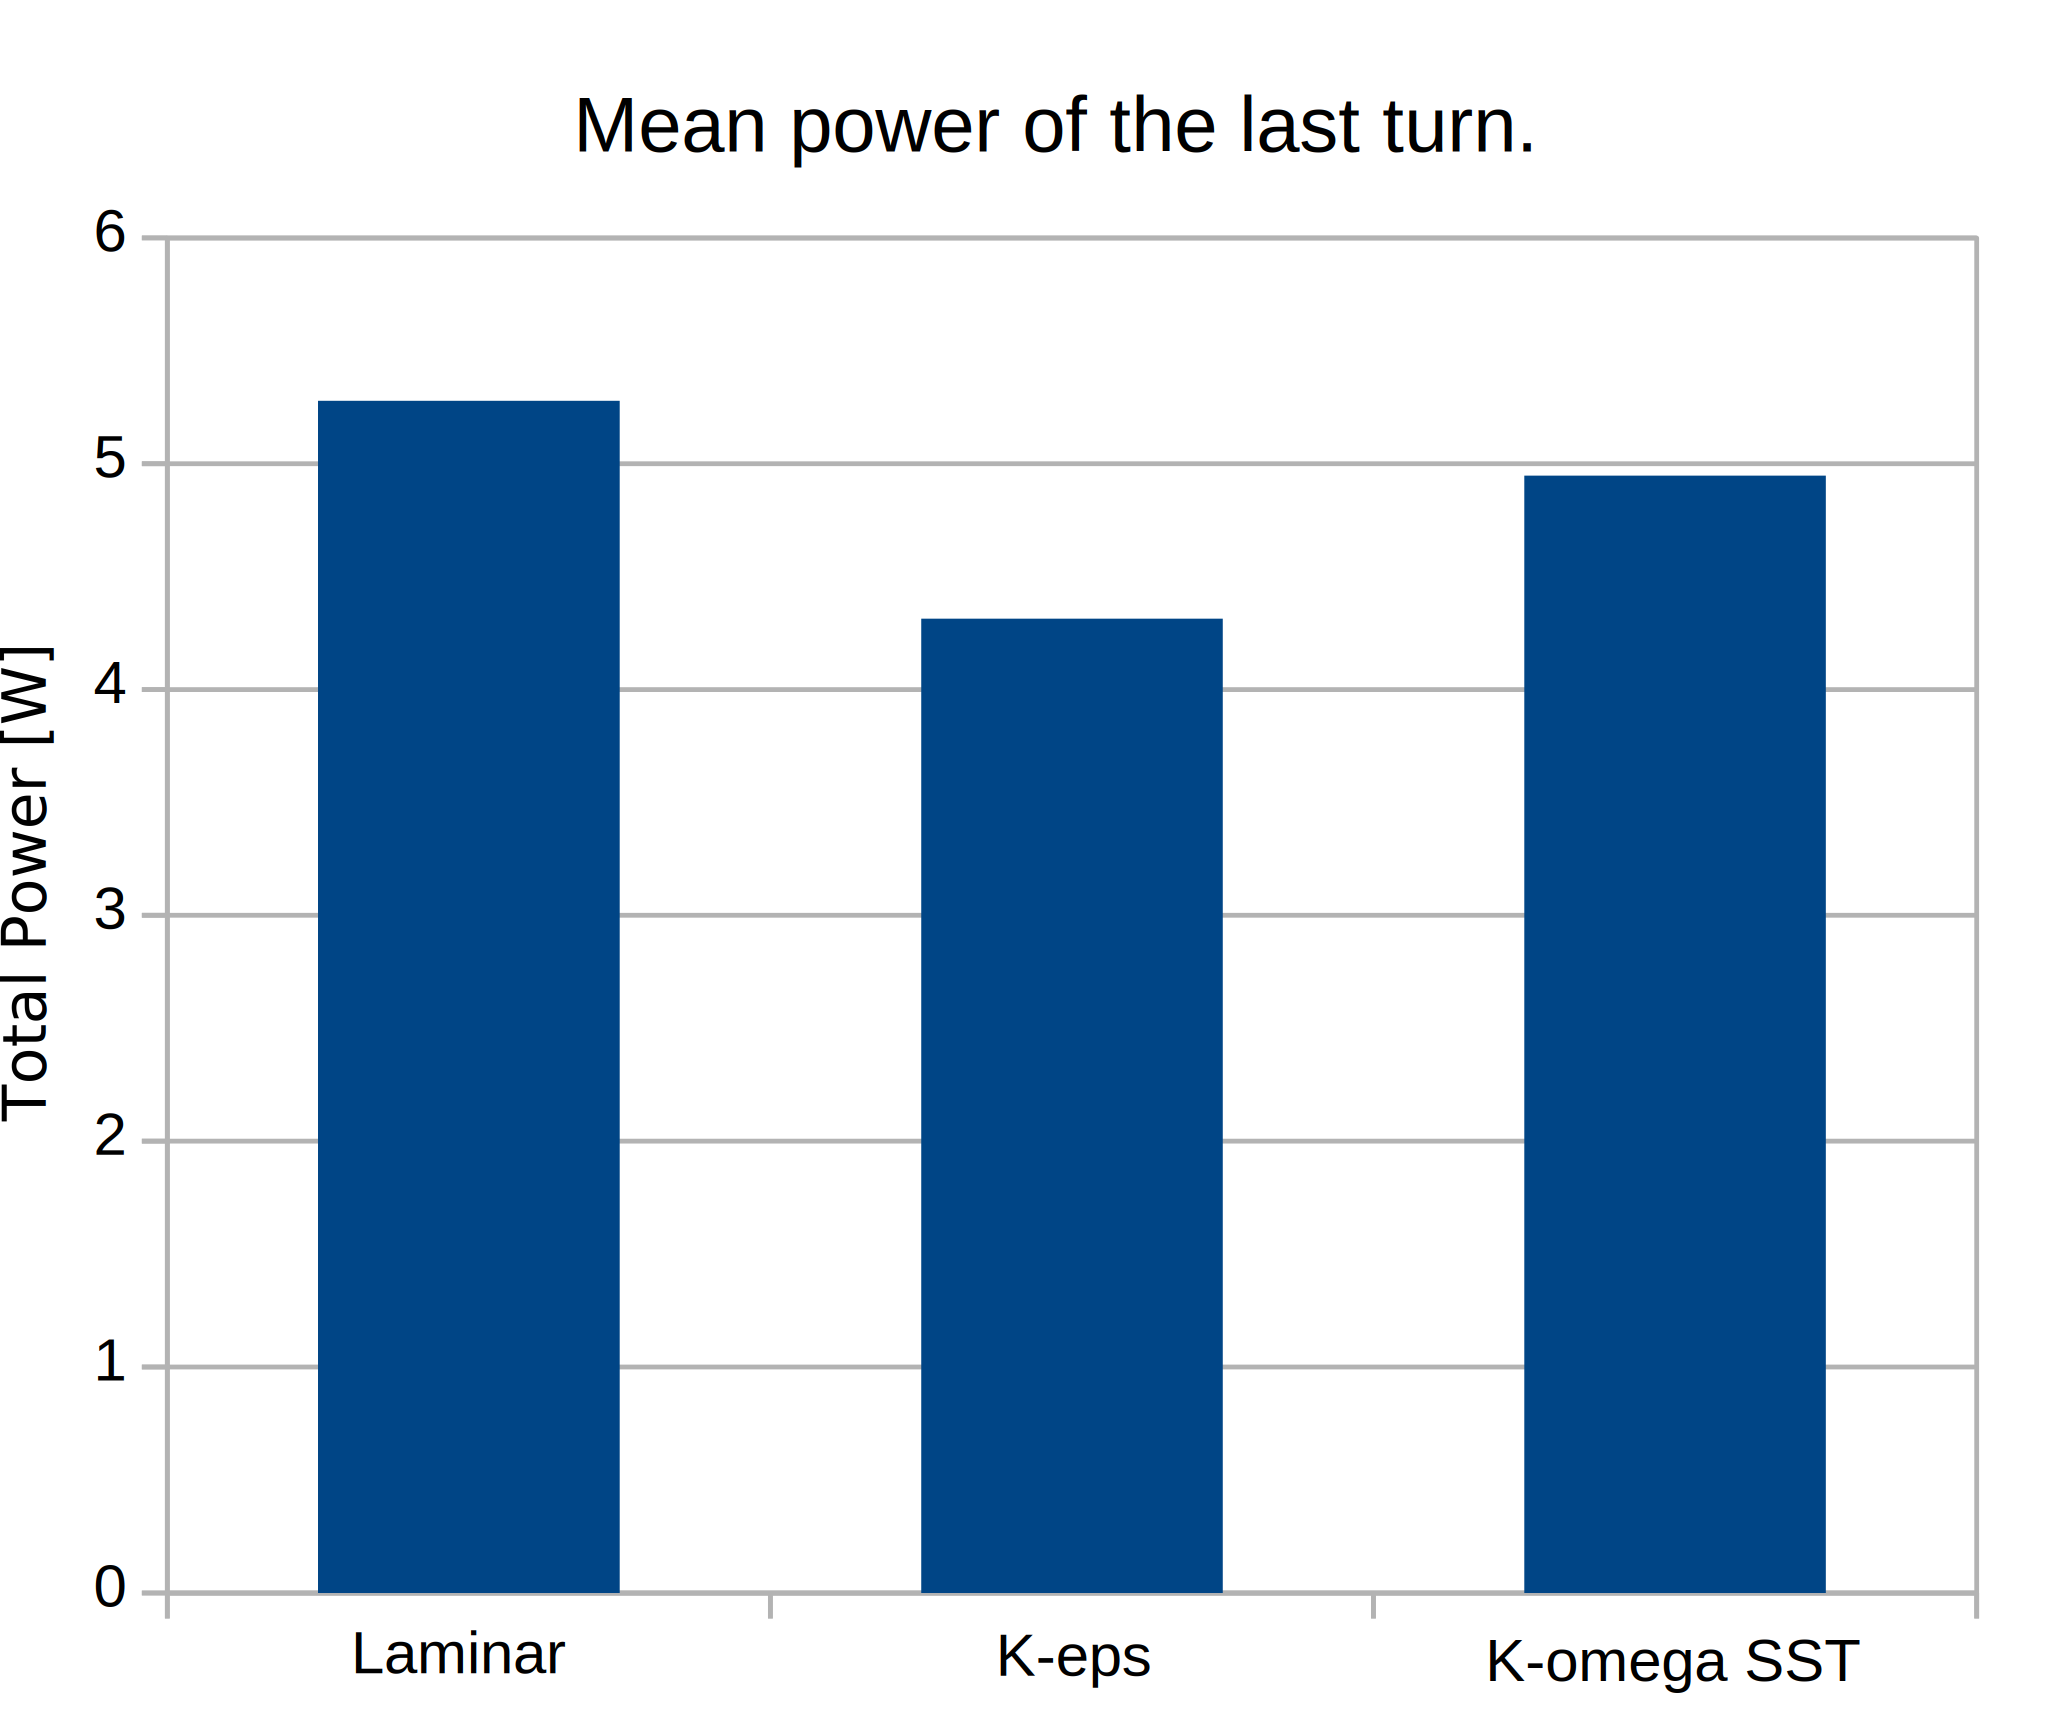
\includegraphics[width=14cm]{images/turbulence/MeanPower_comparison.pdf} 
\caption{total pressure at t = 2.4[s] in a laminar simulation}
\centering
\end{figure}



\paragraph{VELOCITY PROFILES}
As first qualitative reasoning the velocity profiles outcoming from different turbulence simulations have been compared in the wake regions, i.e. where the effect of the turbulence is expected to play its major role.\\
The inspected regions are the following:\\
\begin{figure}[H]
\centering
\subfigure[First section zone: drag wake zone]{\includegraphics[width=8.5cm]{images/turbulence/VerticalBladeWake_screenshot.png}}
\subfigure[Second section zone: mean wake zone]{\includegraphics[width=8.5cm]{images/turbulence/LargeWakeScreenshot.png}}

\end{figure}

\subparagraph{Drag region wake}
First of all it must be noted that on the first velocity section the $k-\varepsilon$ profile results in a different velocity profile with respect to the profiles outcoming from the laminar and $k-\omega SST$ model which, instead have been observed to be quite similar.
The $k-\varepsilon$ profile appears to smear out the velocity gradients which are supposed to be magnified in the viscosity-dominated wake regions.

\begin{figure}[H]
\centering
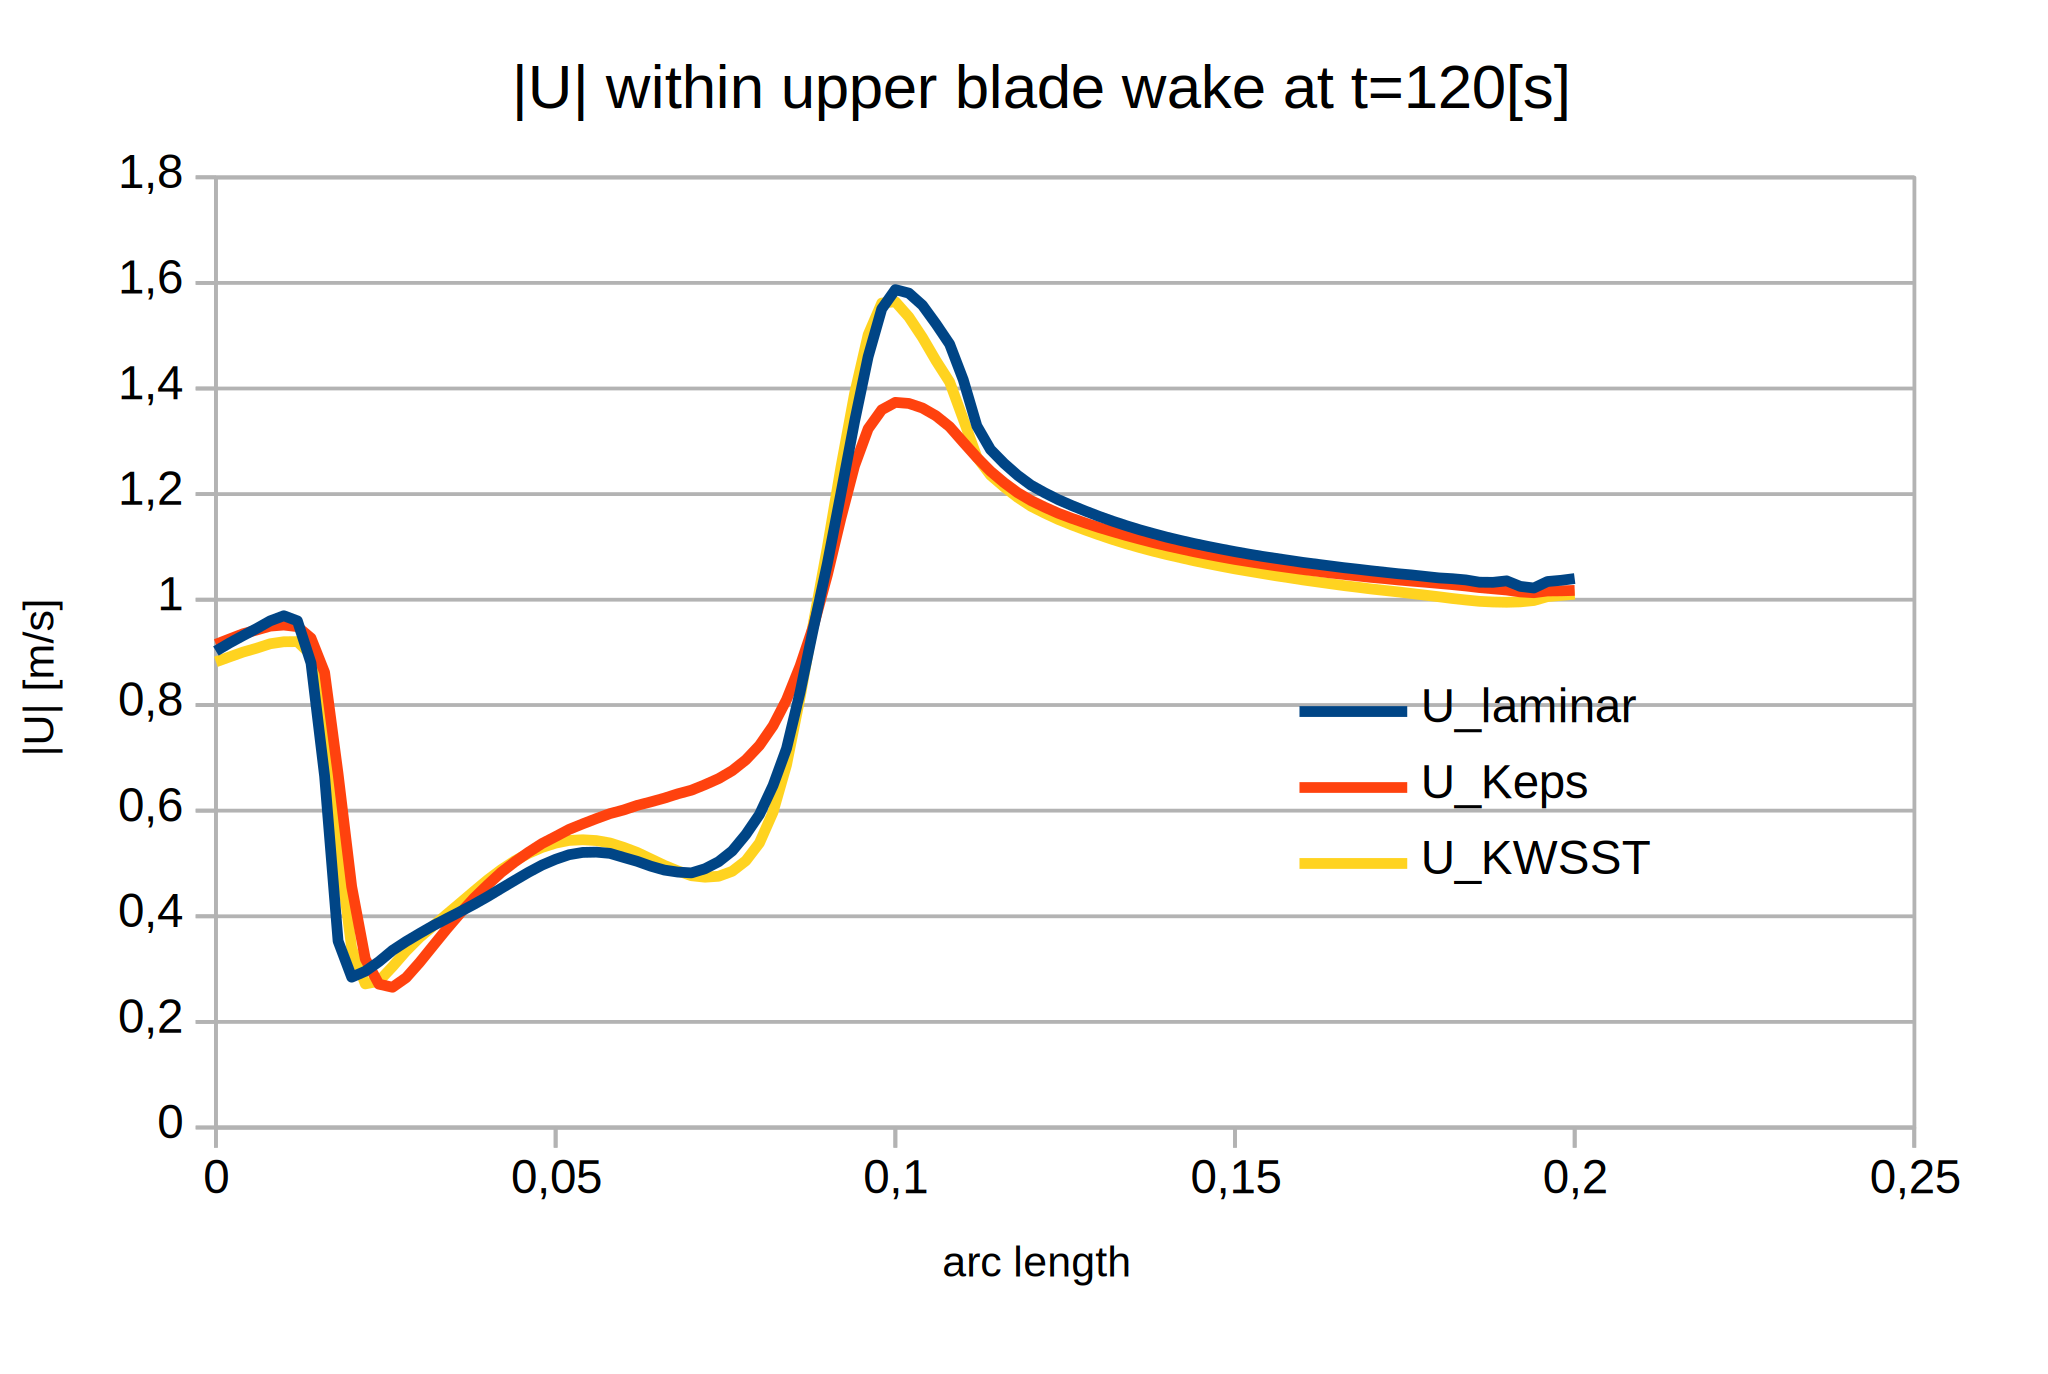
\includegraphics[width=14cm]{images/turbulence/UpperbladeWake.pdf} 
\caption{Velocity profile on the drag-zone wake of the blade}
\centering
\end{figure}

\subparagraph{Large wake region}
On the largest wake section it can be noted again that the difference between velocity profiles is not negligible, in this case it is worth noting that the laminar simulation is that featured by the largest flow deceleration with respect to the upstream profile; this fact could explain the largest mean power extraction that has been found before fo the laminar case.

\begin{figure}[H]
\centering
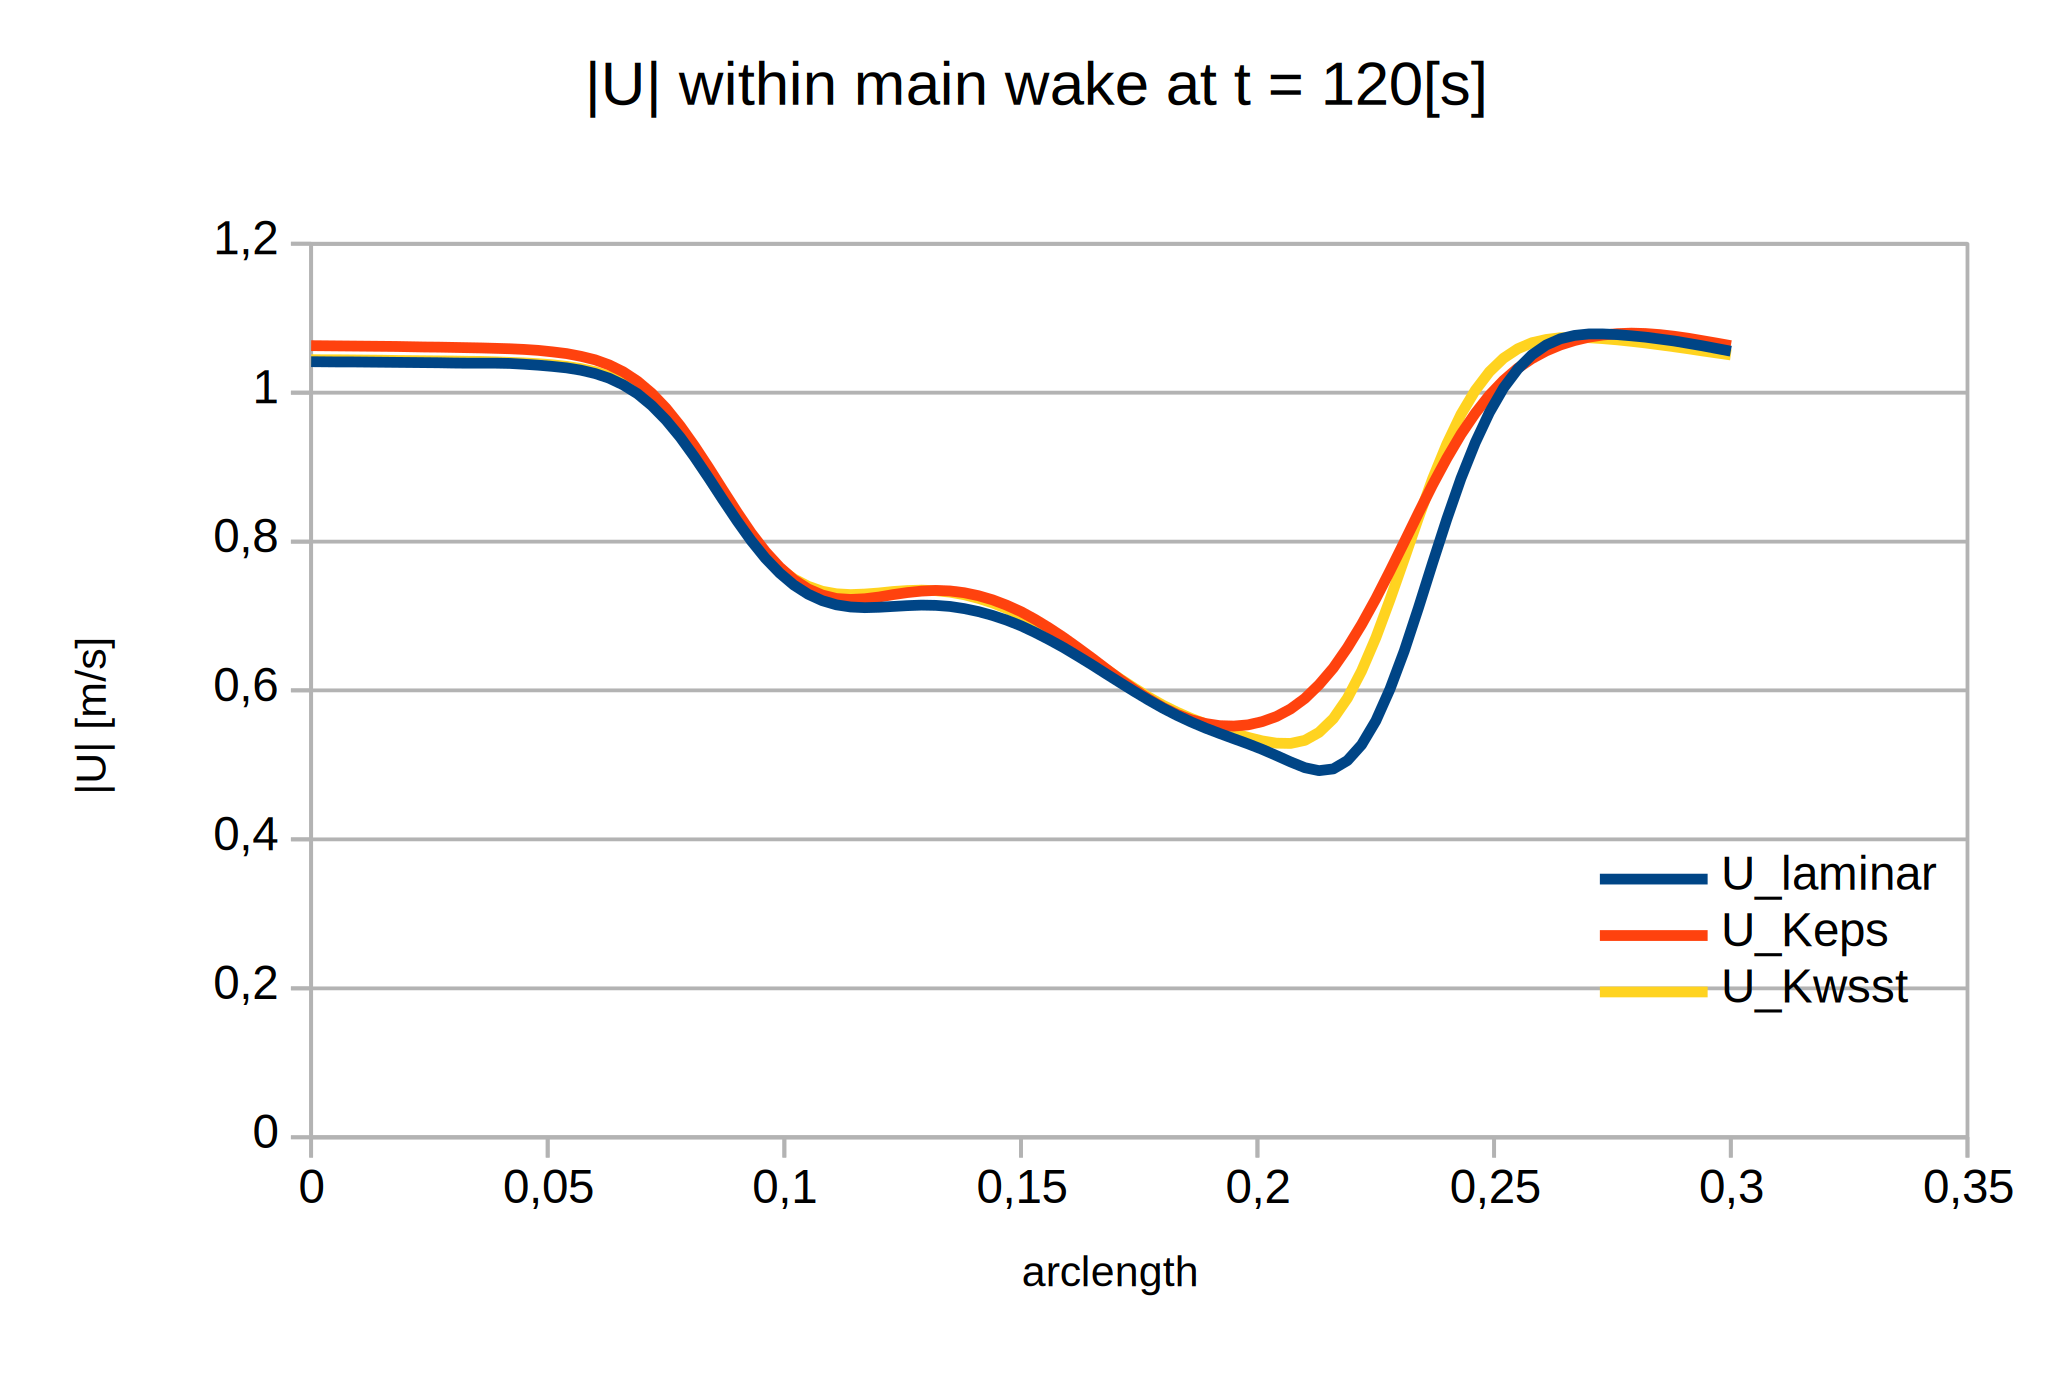
\includegraphics[width=14cm]{images/turbulence/U_mag_MainWake.pdf} 
\caption{Velocity profile on the drag-zone wake of the blade}
\centering
\end{figure}

\subparagraph{Remarks}
From a qualitative point of view it is important to stress the fact that a great accordance has been found between the results of the laminar and the $k-\omega SST$ simulation and instead the $k-\varepsilon$ simulation does not follow the other velocity profiles neither qualitatively.

\subparagraph{Boundary layer}
In order to further clarify this situation, another inspection has been done: the boundary layer on a blade.
The profile has been explored at the time t = 115[s], in correspondance of a null angle of attack of the lower blade with respect to the incoming blade.
Great attention has been paid on the extention of the plot stencil to end within the refinement region.


\begin{figure}[H]
\centering
\includegraphics[width=14cm]{images/turbulence/BL_LowerBlade_screenshot.png} 
\caption{Velocity profile on the drag-zone wake of the blade}
\centering
\end{figure}

The velocity profiles only for the $k-\omega SST$ and $k-\varepsilon$ have been compared.

\begin{figure}[H]
\centering
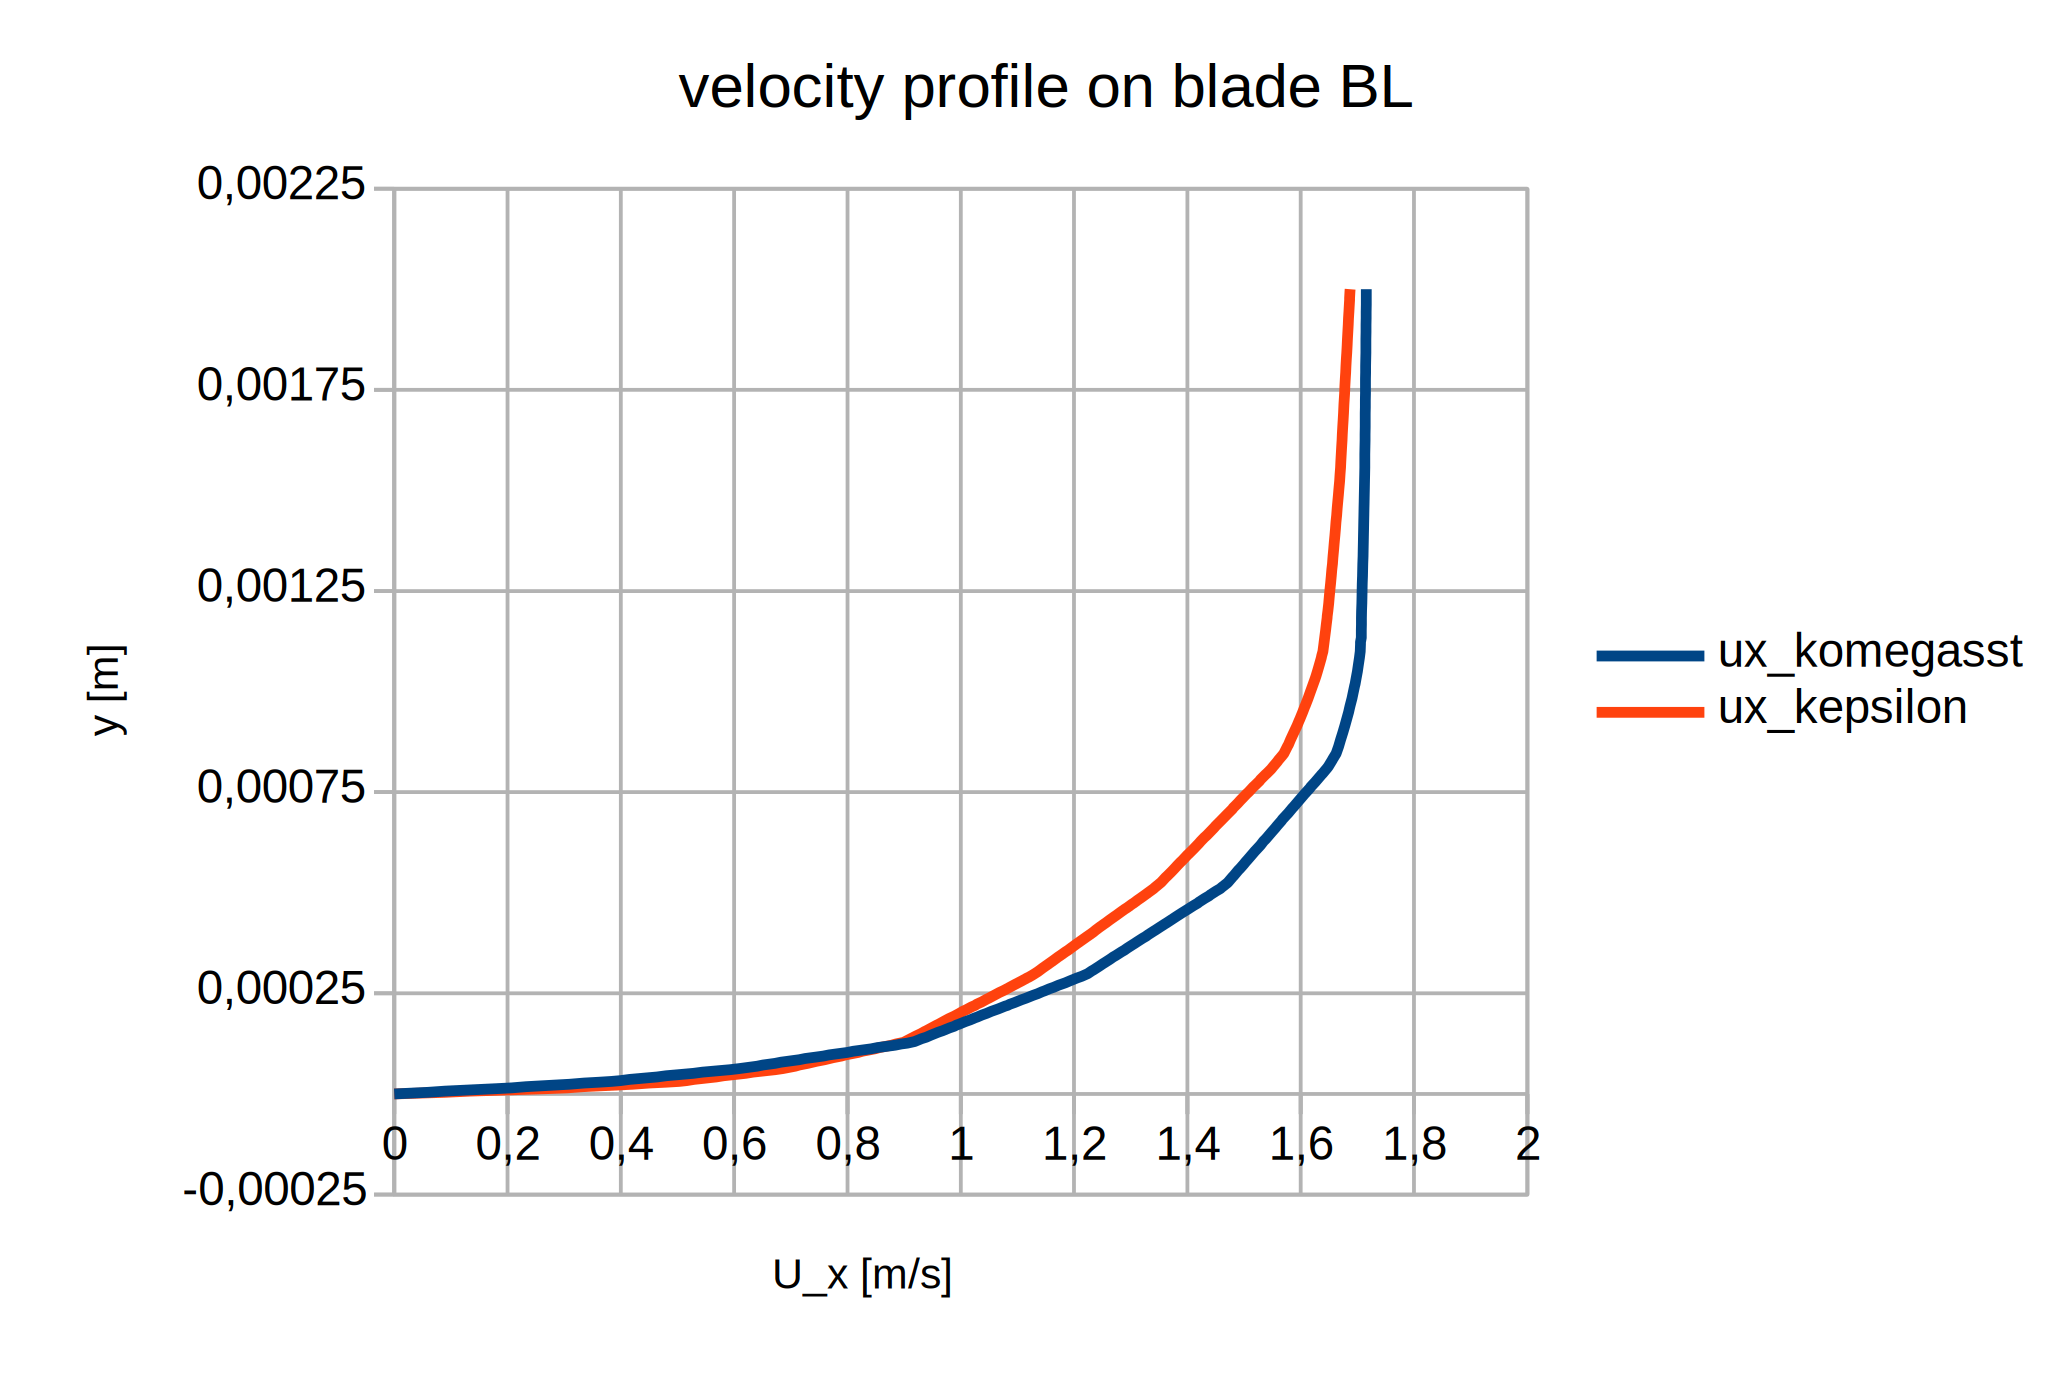
\includegraphics[width=14cm]{images/turbulence/detailBL_kW_Keps.pdf} 
\caption{Velocity profile on the drag-zone wake of the blade}
\centering
\end{figure}

The velocity profiles obtained remark the discrepancy between velocity profiles from the different models.

Then a nondimensional analysis has been carried out on the boundary layer approximation of the $k-\omega SST$ turbulence model.

\begin{figure}[H]
\centering
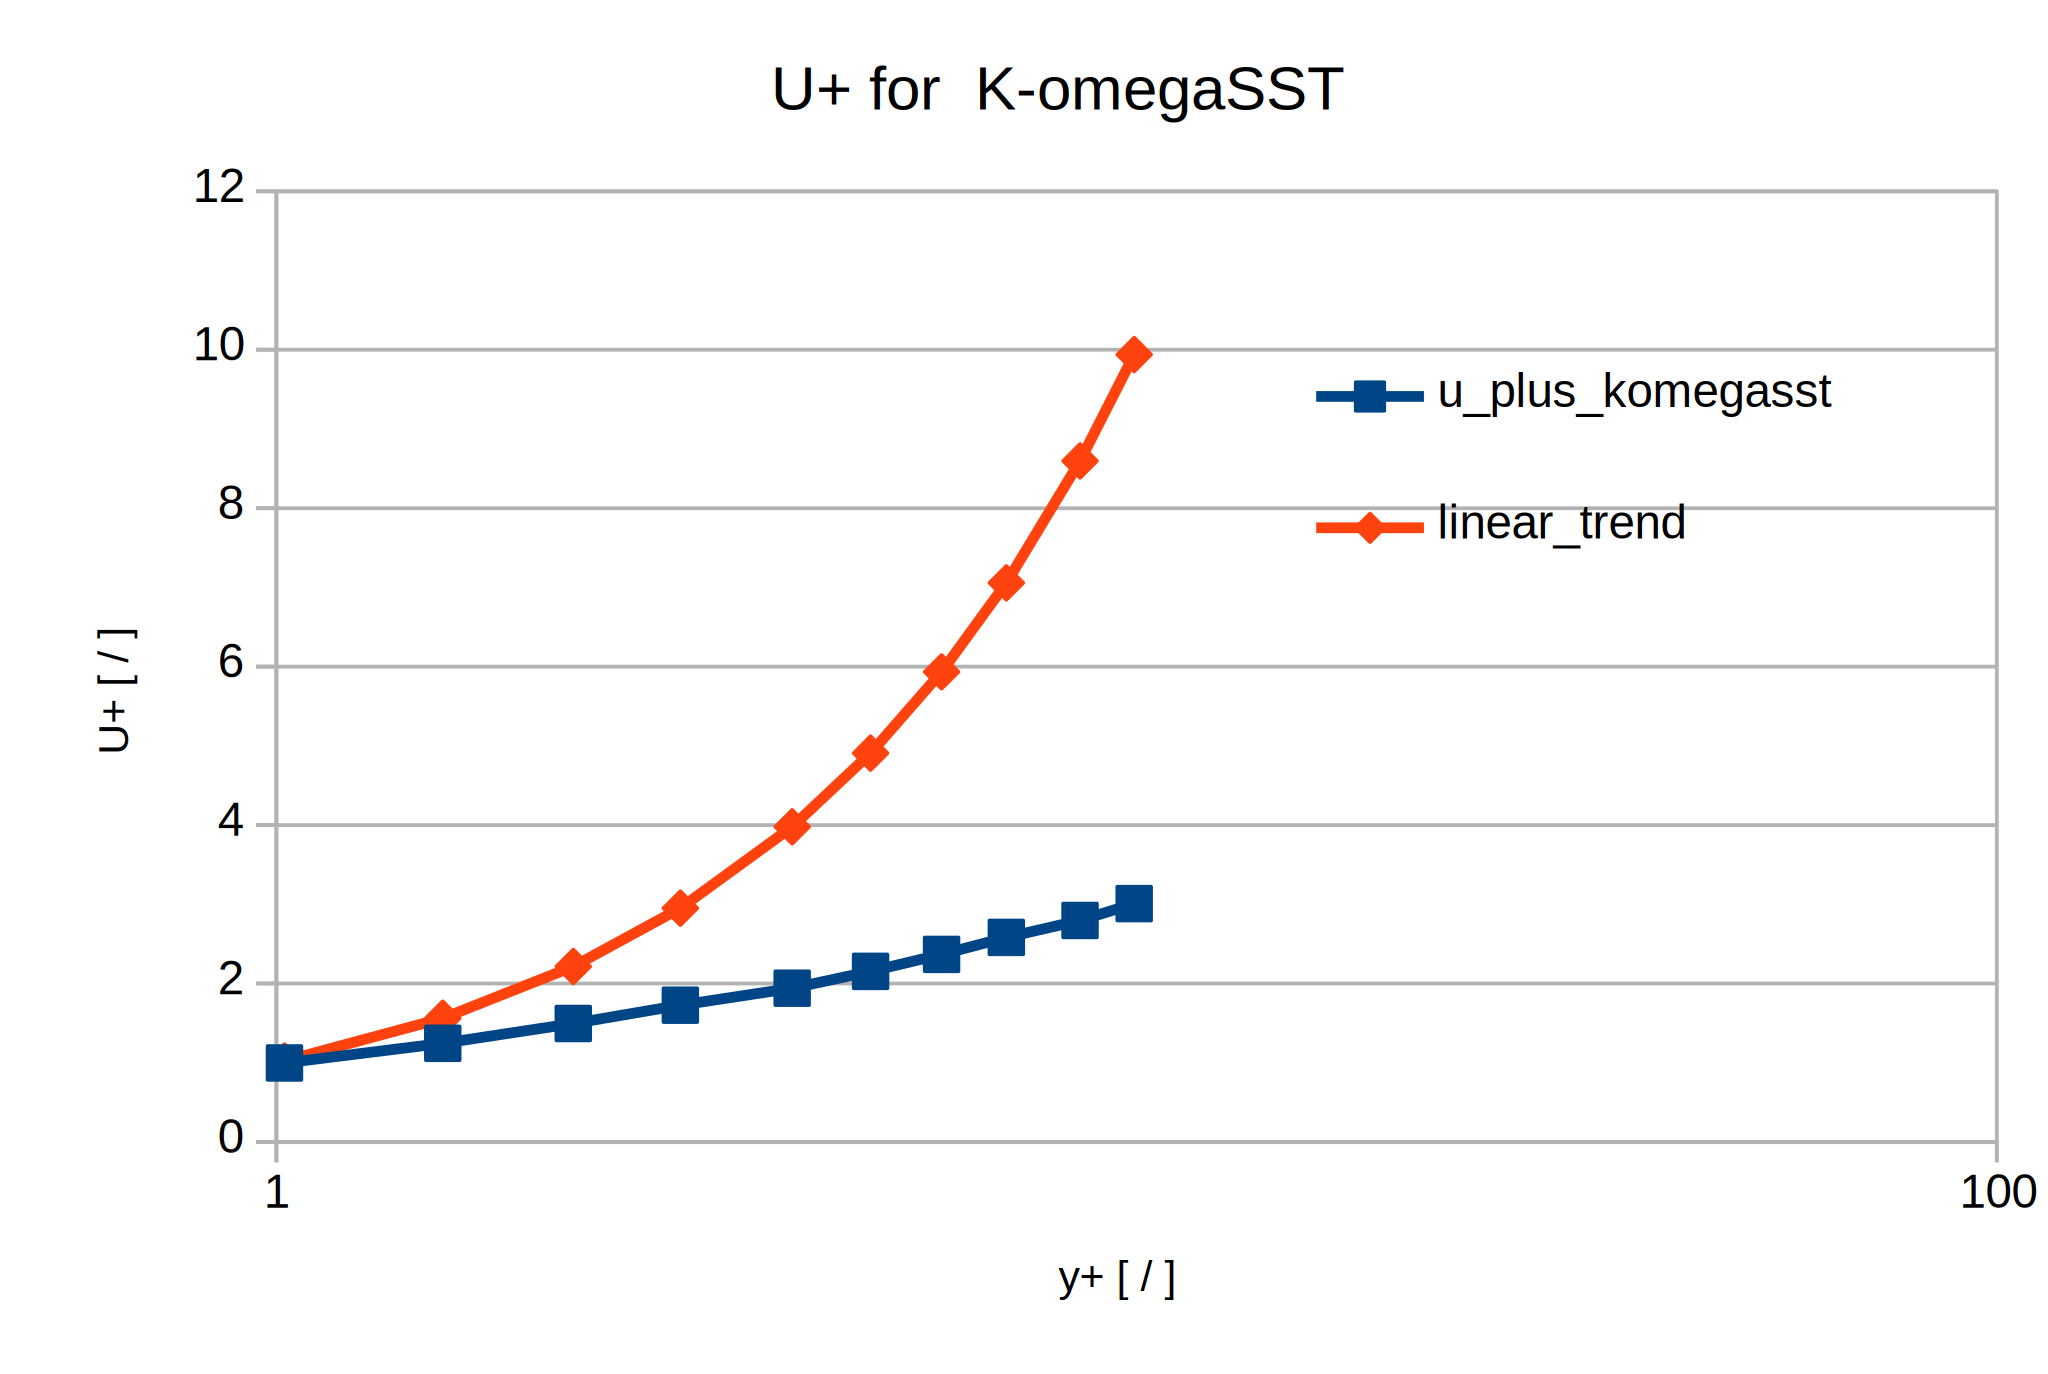
\includegraphics[width=14cm]{images/turbulence/kWsst_BL_sublayer.pdf} 
\caption{Velocity profile on the drag-zone wake of the blade}
\centering
\end{figure}

From the previous results it can be observed that the BL velocity distribution in the linear region is quite different from that developed theoretically for simple shear flow under the assumption of large Reynolds number i.e. thin boundary layer on flat plate.
This trend could probably be justified considering that this particular type of flow displays low Reynolds number which turns out into low turbulence effects.
Only a comparison with experimental results could fully clarify this situation.
The previous hypothesis found its root in the observation of the resemblance of laminar and $k-\omega SST$ velocity profiles.\\
\todo{} PROBABILE STRONZATA

\subsection{flow detatchment}

As previously mentioned, this kind of machine exploit an incompressible flow evolving within aerodynamic profiles with varying angles of attach.
It is straightforward that a good capture of flow detatchment and recirculation are of primary importance.
The $k-\varepsilon$ turbulent model is not suited for capturing the flow detatchment.
The $k-\omega sst$ turbulence model, coupled with a proper refinement strategy near the walls is capable of reproducing the flow detatchment and eventual subsequent recirculation
\includegraphics[width=\textwidth]{images/turbulence/recirculation_scalarScaled.png}

\includegraphics[width=\textwidth]{images/turbulence/recirculation_scalarScaledGOODresolution.png}  

\includegraphics[width=\textwidth]{images/turbulence/recirculation_scalarScaledMESH.png} 

\includegraphics[width=\textwidth]{images/turbulence/recirculation_vectorScaled.png} 

\includegraphics[width=\textwidth]{images/turbulence/recirculation_vectorScaled2.png} 












\end{document}
